\chapter{Formal Analysis Using Alloy}

\section{Alloy Code}

In this section is shown the alloy code that represent some parts of Clup model. The representation focus mainly on how the queue works with different kind of users, from the moment the line-up and so they appear inside this model to the moment they enter inside the store. Their place in the queue is represented by their ticket that encodes inside the QR code the information of lining-up and so of the user. That it is used to recognize the place that a person has in the queue and so to allow only the correct one to enter the store.
It is also shown by the Alloy’s graphic tool some worlds that evidence how the different components of the model and their properties work with each other in different context. And some properties are checked by using the assertion feature. 


\lstinputlisting[language=Alloy]{alloy/Clup_final.als}

\begin{figure}[H]
	\centering
	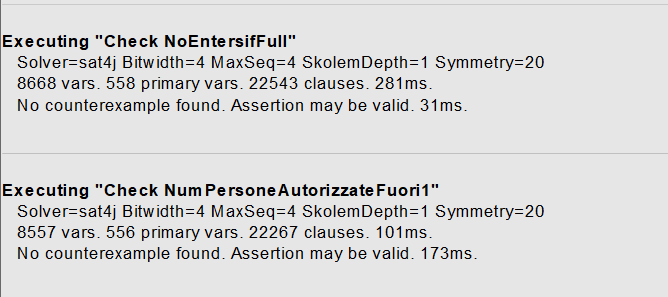
\includegraphics[width=\textwidth]{images/Assertions.png}
	\caption{Assertions verification}
	\label{figure: Assertions verification}
\end{figure}

\begin{sidewaysfigure}
	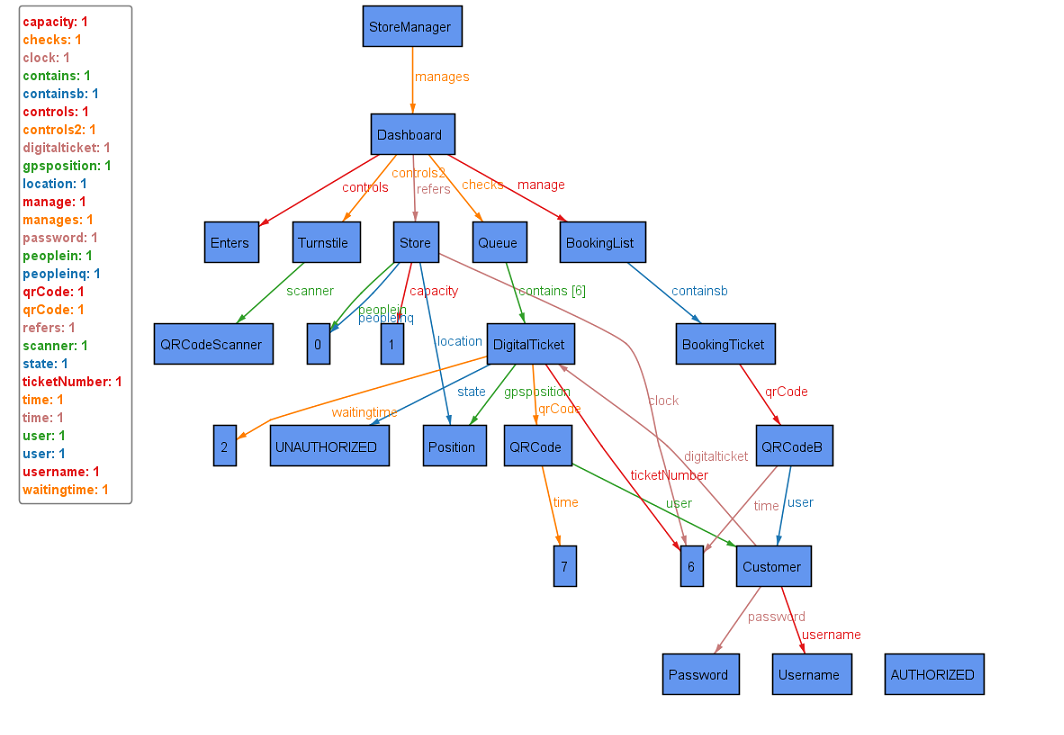
\includegraphics[width=1.0\textwidth]{images/AlloyW1.png}
	\caption{World1.}
	\label{figure: World1}
\end{sidewaysfigure}

\begin{sidewaysfigure}
	\centering
	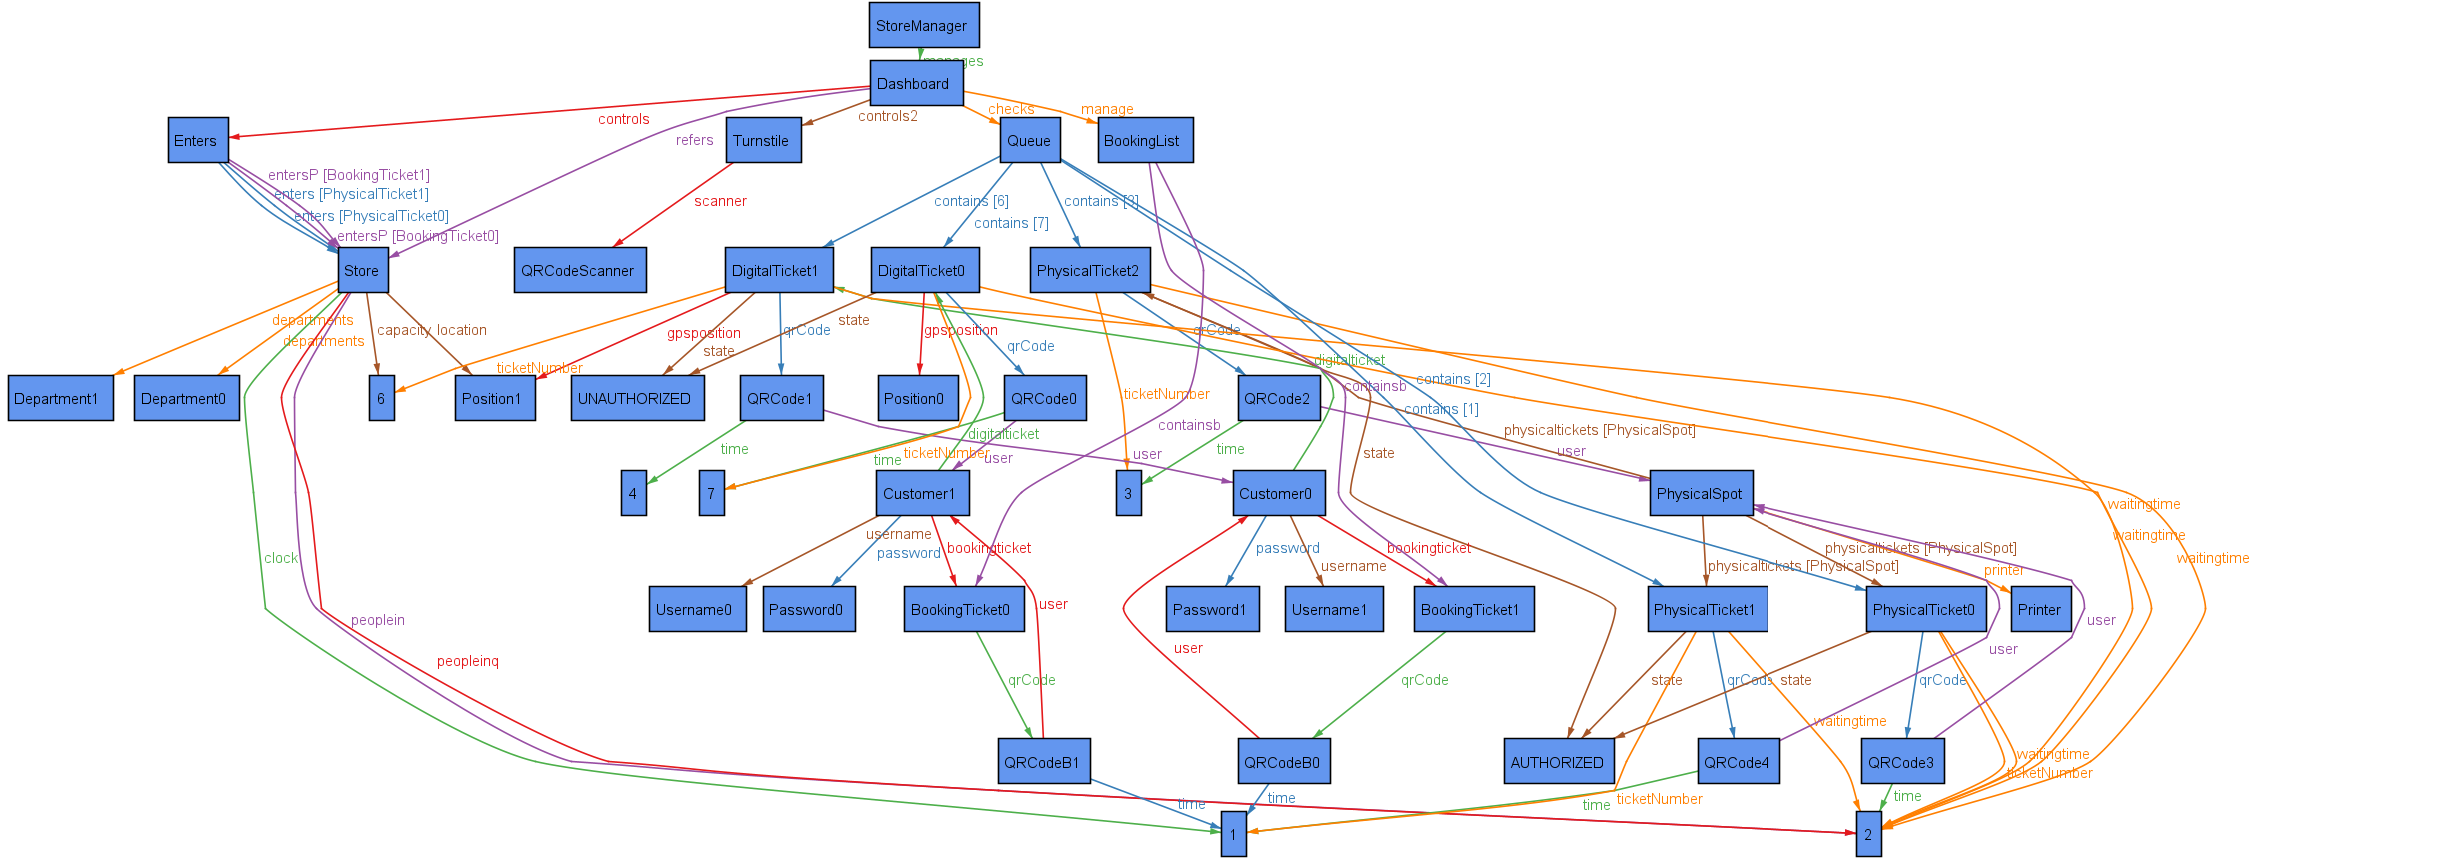
\includegraphics[width=1.0\textwidth]{images/world_3.png}
	\caption{World2.}
	\label{figure: World2}
\end{sidewaysfigure}

\begin{sidewaysfigure}
	\centering
	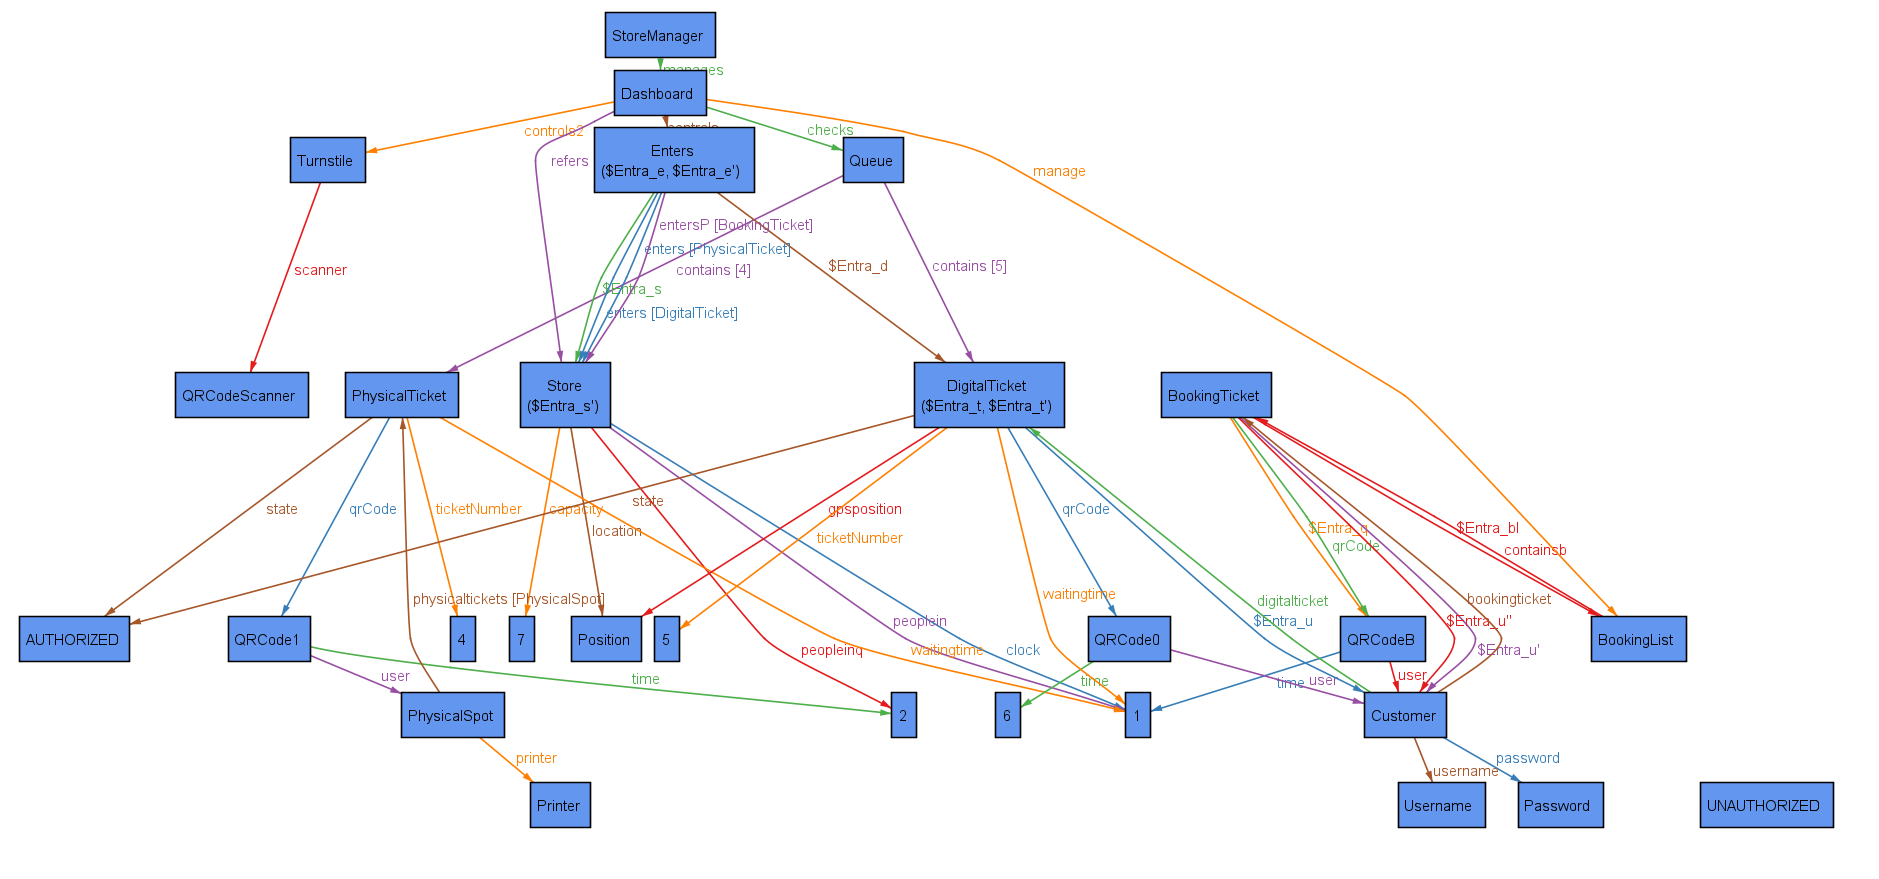
\includegraphics[width=1.0\textwidth]{images/EntraFunction}
	\caption{Entra function.}
	\label{figure: Entra function}
\end{sidewaysfigure}